\chapter{Inleiding}
\chapterpreamble

%
%
%
\section{Productomschrijving}

De \product is een set van twee cartridges waarmee SD-kaartjes uitgelezen kunnen worden op de \pkb{P2000T} of \pkb{P2000M} en programma's ingeladen in het geheugen. Vervolgens kunnen deze programma's opgestart worden. De \product is een datadrager die vergelijkbaar met het cassettedeck of een floppydrive en welke cassette bestanden (\cas) kan inladen en opstarten in een BASICNL v1.1 omgeving. Wanneer de \pkb{P2000T} voorzien is van tenminste een 16 KiB geheugenuitbreiding kan de P2000T ook machinetaalbestanden (\prg) inladen in het geheugenblok \pkb{0xA000-0xDFFF} en opstarten.

%
%
\subsection{Technische specificaties}

\begin{itemize}[noitemsep]
    \item 16 MHz klok-generator
    \item 128 KiB alleen-lezen geheugen (ROM)
    \item 128 KiB schrijfbaar geheugen (RAM)
    \item SD-kaart houder met 5V naar 3.3V spanningsomvormer en bidirectionele niveauregelaar
    \item 2 x 8-bit registers voor de adresbus van de ROM en RAM chips
    \item 1 x 2-bit register voor bankselectie van de ROM en RAM chips (2 x 64 KiB banken)
    \item 2 schuifregisters voor data-communicatie met de SD-kaart
\end{itemize}

%
%
%
\section{Cartridges}

De \product is een set van twee cartridges: een \sleuf{1} en \sleuf{2} cartridge. De \sleuf{1} cartridge heeft aan de voorzijde een DIP schakelaar, de \sleuf{2} cartridge heeft aan de voorzijde 4 LED-lampjes\index{LED-lampjes}. Over het algemeen wordt de \sleuf{1} cartridge geleverd met een zwart-oranje behuizing en de \sleuf{2} cartridge met een zwart-witte behuizing.

%
%
%
\subsection{Sleuf 1 cartridge}

\index{Sleuf 1 cartridge}
\index{SLOT 1 cartridge|see{Sleuf 2 cartridge}}

Cartridge 1 (zwart-oranje) is een \sleuf{1} multirom cartridge (zie \cref{fig:cartridge-sleuf1}) waarbij de gebruiker middels een DIP schakelaar aan de voorzijde van de cartridge de gewenste ROM kan selecteren.

\begin{figure}[h!]
    \centering
    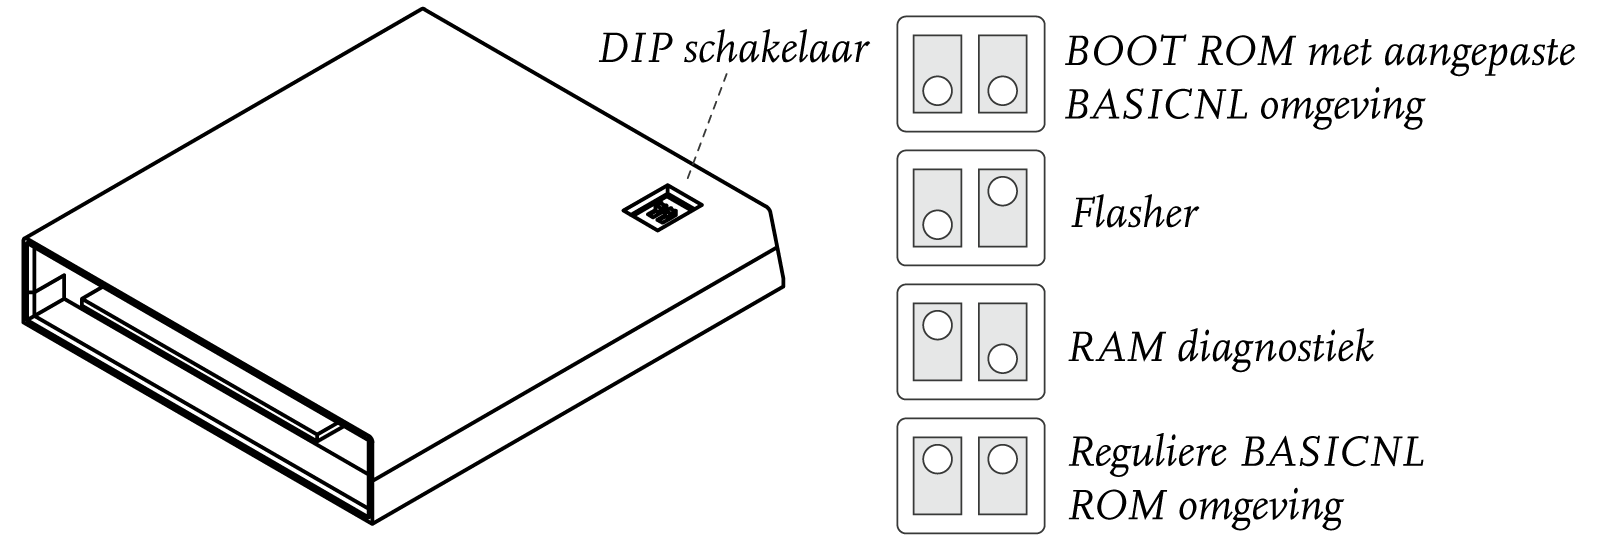
\includegraphics[width=0.99\textwidth]{img/slot1-cartridge.png}
    \caption{Sleuf 1 cartridge. Middels de DIP schakelaar kan het gewenste ROM geselecteerd worden.}
    \label{fig:cartridge-sleuf1}
\end{figure}

De cartridge bevat een 64 KiB ROM chip waardoor op deze (enkele) cartridge de inhoud van vier reguliere cartridges (4 x 16 KiB) geplaatst kan worden. De volgende cartridge-roms zijn op de \sleuf{1} cartridge aanwezig:

\begin{enumerate}[noitemsep]
    \item Aangepaste BASICNL v1.1 om cassette bestanden op te kunnen starten. (zie \cref{chap:usage})
    \item Flash programma om de firmware op Cartridge 2 (zwart-wit) te kunnen updaten. (zie \cref{sec:firmware-flash})
    \item Geheugen test om te controleren of het geheugen in de \pkb{P2000T} inclusief eventuele geheugenuitbreidingen correct functioneren.
    \item Kopie van de reguliere BASICNL v1.1 cartridge voor als de gebruiker de P2000T in de reguliere BASICNL omgeving wilt opstarten.
\end{enumerate}

%
%
%
\subsection{Sleuf 2 cartridge}

\index{Sleuf 2 cartridge}
\index{SLOT 2 cartridge|see{Sleuf 2 cartridge}}

Cartridge 2 (zwart / wit) is een \sleuf{2} cartridge (zie \cref{fig:cartridge-sleuf2}) met de benodigde schakelingen zodat de \pkb{P2000T} kan communiceren met het SD kaartje. Deze cartridge bevat naast een SD-kaart houder, ook een 128 KiB ROM chip (SST39SF010) en een 128 KiB RAM chip (62128). De ROM chip wordt gebruikt om de firmware op te slaan terwijl de RAM chip gebruikt wordt als buffer zodat grote stukken data opgeslagen kunnen worden zonder het interne geheugen van de \pkb{P2000T}, welke vaak relatief beperkt is, te belasten.

\begin{figure}[h!]
    \centering
    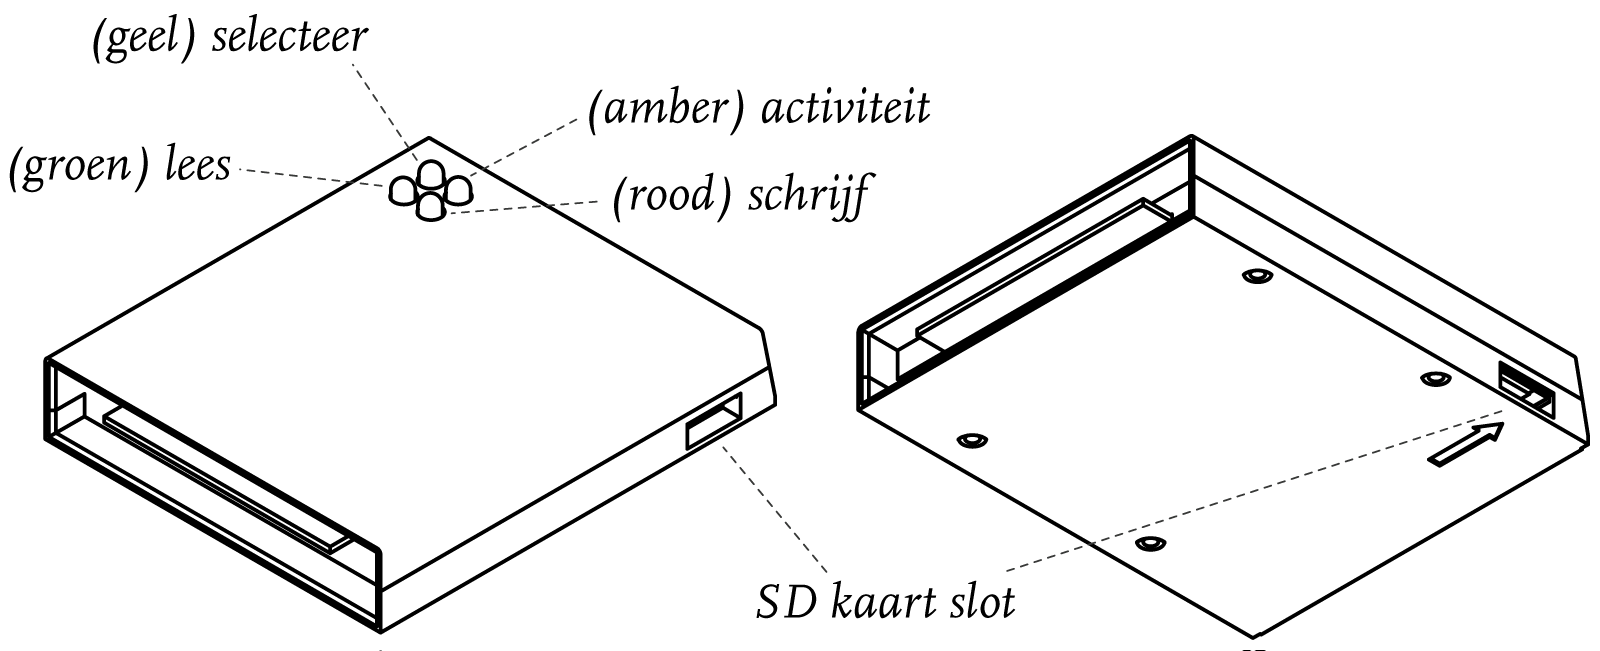
\includegraphics[width=0.99\textwidth]{img/sd-card-cartridge.png}
    \caption{Sleuf 2 cartridge. Vier LED-lampjes aan de bovenzijde (linker afbeelding) geven de operaties op de cartridge aan. Aan de onderzijde (rechter afbeelding) geeft een pijl de uitsparing voor de SD-kaart lezer aan.}
    \label{fig:cartridge-sleuf2}
\end{figure}

Aan de voorzijde van de cartridge bevinden zich 4 LED-lampjes. Deze geven de lopende operaties van de cartridge aan.

\begin{itemize}[noitemsep]
    \item \pkb{Geel}: De SD-kaart is geactiveerd.
    \item \pkb{Amber}: Er is data-overdracht tussen de SD-kaart en de \pkb{P2000T}.
    \item \pkb{Groen}: Er wordt vanaf de cartridge gelezen. Deze lees-operaties zijn naar de ROM of RAM chip.
    \item \pkb{Rood}: Er wordt data naar de cartridge geschreven. Deze schrijf-operaties zijn naar de ROM of naar de RAM chip.
\end{itemize}

%
%
%
\section{Broncode, schema's en licentie}

\index{licentie}
\index{broncode}

De \product is een volledig open-source en open-hardware product. De bronbestanden om de PCBs te fabriceren en de broncode voor de software zijn te verkrijgen via deze Github repository:\\ \faGithub \;\url{https://github.com/ifilot/p2000t-sdcard/}.

De software wordt gedistribueerd onder een GPLv3\footnote{\url{https://www.gnu.org/licenses/gpl-3.0.en.html}} licentie. De hardware valt onder een CC-BY-SA\footnote{\url{https://creativecommons.org/licenses/by-sa/4.0/deed.en}} licentie.